
\title{SOS and SOSflow: Scalable Observation System for Complex High-Performance Applications}

%\author{\IEEEauthorblockN{Chad Wood}
%        \IEEEauthorblockN{Daniel Ellsworth}
%        \IEEEauthorblockN{Sudhanshu Sane}
%	\IEEEauthorblockN{Kevin Huck}
%        \IEEEauthorblockN{Allen Malony}
\author{\IEEEauthorblockN{Chad Wood, Daniel Ellsworth, Sudhanshu Sane, Kevin Huck, Allen Malony}
        \IEEEauthorblockA{Department of Computer and Information Science\\
                          University of Oregon\\
                          Eugene, OR United States\\
        Email: \{cdw,dellsworth,ssane,khuck,malony\}@cs.uoregon.edu} }

\maketitle


\begin{abstract}
%%%%%
The Scalable Observation System (SOS) introduces a new workflow
runtime system (SOSflow) to enable online in situ characterization and
analysis of complex high-performance computing applications.
%
SOS emphasizes a semantic data model with distributed information
management and structured query and access.
%
The primary design objectives of SOSflow are flexibility, scalability,
and programmability, with data being annotated for use in high-level
reasoning about total scientific workflow performance from a variety
of perspectives.
%
SOSflow provides a complete framework that can be configured with and
used directly by an application, allowing for simultaneous semantic
encoding of multiple observation sources as well as analytics modules
that can operate over information provided by any and all contributing
sources.

\fix{Sudhanshu version - 
%%%%%
The Scalable Observation System (SOS) introduces a new 
runtime system (SOSflow) to enable online in situ characterization and
analysis of complex high-performance computing applications.
%
SOS employs a data model with distributed information
management and structured query and access capabilities.
%
The primary design objectives of SOSflow system are flexibility, scalability,
and programmability. 
%
SOSflow provides a complete framework that can be configured with and 
used directly be an application, allowing for a detailed workflow analysis of scientific applications. 
%
---- Two three lines about the paper ---- What this paper observed --- that this system is on par with existing technologies --- it provides improvement over other technologies --- something along these lines.
%%%%
}

%%%%%
\end{abstract}


\begin{IEEEkeywords}
hpc; exascale; in situ; performance; monitoring; introspection;
monalytics; scientific workflow; sos; sosflow;
\end{IEEEkeywords}


\IEEEpeerreviewmaketitle


\begin{figure*}[!t]
\centering
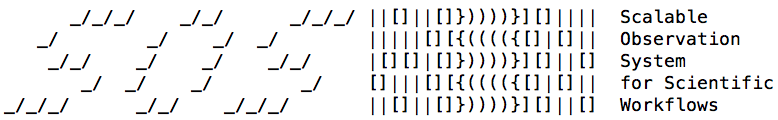
\includegraphics[width=5in]{images/sosflow_masthead.png}
%\caption{SOSflow: Overview}
\label{fig_sim}
\end{figure*}



%\todofileend{010\_title\_authors.tex}
